% ===========================================================================
%  TikuOS — Building, Toolchain Setup & Architecture
%  Beamer Presentation
% ===========================================================================
\documentclass[aspectratio=169, 10pt]{beamer}

% ---- Theme ----------------------------------------------------------------
\usetheme{Madrid}
\usecolortheme{whale}
\setbeamertemplate{navigation symbols}{}
\setbeamertemplate{footline}{%
  \leavevmode\hbox{%
    \begin{beamercolorbox}[wd=.33\paperwidth,ht=2.5ex,dp=1ex,center]{author in head/foot}%
      \usebeamerfont{author in head/foot}\insertshortauthor
    \end{beamercolorbox}%
    \begin{beamercolorbox}[wd=.34\paperwidth,ht=2.5ex,dp=1ex,center]{title in head/foot}%
      \usebeamerfont{title in head/foot}\insertshorttitle
    \end{beamercolorbox}%
    \begin{beamercolorbox}[wd=.33\paperwidth,ht=2.5ex,dp=1ex,right]{date in head/foot}%
      \usebeamerfont{date in head/foot}\insertshortdate{}\hspace*{2em}%
      \insertframenumber{}/\inserttotalframenumber\hspace*{2ex}
    \end{beamercolorbox}}%
  \vskip0pt%
}

% ---- Packages -------------------------------------------------------------
\usepackage{listings}
\usepackage{graphicx}
\usepackage{hyperref}
\usepackage{booktabs}
\usepackage{tikz}
\usetikzlibrary{arrows.meta, positioning, shapes.geometric, fit}

% ---- Code listing style ---------------------------------------------------
\lstset{
  basicstyle=\ttfamily\scriptsize,
  keywordstyle=\color{blue}\bfseries,
  commentstyle=\color{gray},
  stringstyle=\color{red!70!black},
  showstringspaces=false,
  breaklines=true,
  frame=single,
  rulecolor=\color{black!30},
  backgroundcolor=\color{blue!3},
  tabsize=4,
}
\lstdefinestyle{makestyle}{
  language=make,
  morekeywords={make,MCU,DEBUGGER,PORT,BAUD},
}
\lstdefinestyle{cstyle}{
  language=C,
  morekeywords={uint8_t,uint16_t,uint32_t,tiku_process_t,tiku_clock_time_t},
}
\lstdefinestyle{bashstyle}{
  language=bash,
  morekeywords={sudo,apt,wget,tar,export,make},
}

% ---- Metadata -------------------------------------------------------------
\title[TikuOS]{TikuOS}
\subtitle{Simple. Ubiquitous. Intelligence, Everywhere.}
\author[Ambuj Varshney]{Ambuj Varshney \\ \texttt{ambuj@tiku-os.org}}
\date{\today}

% ===========================================================================
\begin{document}

% ---------------------------------------------------------------------------
\begin{frame}
\titlepage
\end{frame}

% ---------------------------------------------------------------------------
\begin{frame}{Outline}
\tableofcontents
\end{frame}

% ===========================================================================
\section{Introduction}
% ===========================================================================

\begin{frame}{What is TikuOS?}
\begin{itemize}
  \item Event-driven embedded OS for \textbf{ultra-low-power} MSP430 microcontrollers
  \item Cooperative multitasking via \textbf{protothreads}
  \item \textbf{Zero dynamic allocation} — all memory is statically managed
  \item Targets MSP430 FRAM variants: FR5969, FR5994, FR2433
  \item Apache 2.0 licensed
\end{itemize}

\vspace{0.5em}
\begin{block}{Key Design Principles}
\begin{itemize}
  \item Minimal footprint for 2--256\,KB FRAM, 2--8\,KB RAM
  \item Hardware abstraction: device headers + board headers
  \item Single unified Makefile supporting all MCU variants
\end{itemize}
\end{block}
\end{frame}

% ---------------------------------------------------------------------------
\begin{frame}{Supported Hardware}
\begin{table}
\centering
\small
\begin{tabular}{@{}lccc@{}}
\toprule
\textbf{Feature} & \textbf{FR2433} & \textbf{FR5969} & \textbf{FR5994} \\
\midrule
RAM              & 4\,KB   & 2\,KB   & 8\,KB    \\
FRAM             & 16\,KB  & 64\,KB  & 256\,KB  \\
Max Clock        & 16\,MHz & 8\,MHz  & 16\,MHz  \\
GPIO Ports       & P1--P3  & P1--P4, PJ & P1--P8, PJ \\
LFXT Crystal     & No      & Yes     & Yes      \\
HFXT Crystal     & No      & Yes     & Yes      \\
\bottomrule
\end{tabular}
\end{table}

\vspace{0.3em}
\begin{alertblock}{Default Target}
If no \texttt{MCU=} is specified, the build defaults to \textbf{MSP430FR2433}.
\end{alertblock}
\end{frame}

% ===========================================================================
\section{Project Structure}
% ===========================================================================

\begin{frame}[fragile]{Directory Layout}
\begin{columns}[T]
\begin{column}{0.48\textwidth}
\begin{lstlisting}[basicstyle=\ttfamily\tiny, frame=none]
tikuOS/
|-- Makefile            # Universal build
|-- main.c              # Entry point
|-- tiku.h              # Master config
|-- arch/msp430/
|   |-- tiku_device_select.h
|   |-- devices/
|   |   |-- tiku_device_fr5969.h
|   |   |-- tiku_device_fr5994.h
|   |   +-- tiku_device_fr2433.h
|   +-- boards/
|       |-- tiku_board_fr5969_launchpad.h
|       |-- tiku_board_fr5994_launchpad.h
|       +-- tiku_board_fr2433_launchpad.h
\end{lstlisting}
\end{column}
\begin{column}{0.48\textwidth}
\begin{lstlisting}[basicstyle=\ttfamily\tiny, frame=none]
|-- kernel/
|   |-- process/        # Protothreads
|   |-- timers/         # Clock, htimer, timer
|   |-- scheduler/      # Event loop
|   +-- memory/         # Arena allocator
|-- boot/               # Boot sequence
|-- hal/                # CPU HAL
|-- tests/              # Test framework
|-- examples/           # 9 example apps
|   |-- 01_blink/
|   |-- 02_dual_blink/
|   |-- ...
|   +-- 09_channel/
+-- docs/               # Documentation
\end{lstlisting}
\end{column}
\end{columns}
\end{frame}

% ---------------------------------------------------------------------------
\begin{frame}[fragile]{Architecture Overview}
\begin{center}
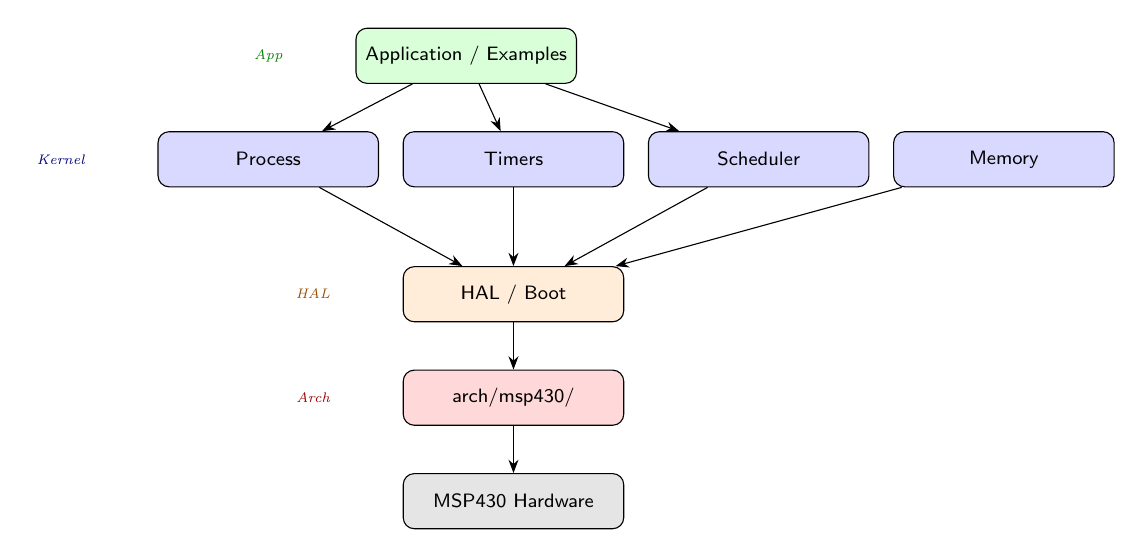
\begin{tikzpicture}[
    box/.style={draw, rounded corners, minimum width=2.8cm, minimum height=0.7cm,
                text centered, font=\scriptsize\sffamily},
    layer/.style={draw, dashed, rounded corners, inner sep=6pt, fill=#1},
    >=Stealth,
    node distance=0.4cm
  ]
  % Application layer
  \node[box, fill=green!15] (app) {Application / Examples};

  % Kernel layer
  \node[box, fill=blue!15, below left=0.6cm and -0.3cm of app] (proc) {Process};
  \node[box, fill=blue!15, right=0.3cm of proc] (timer) {Timers};
  \node[box, fill=blue!15, right=0.3cm of timer] (sched) {Scheduler};
  \node[box, fill=blue!15, right=0.3cm of sched] (mem) {Memory};

  % HAL
  \node[box, fill=orange!15, below=1.0cm of timer] (hal) {HAL / Boot};

  % Arch
  \node[box, fill=red!15, below=0.6cm of hal] (arch) {arch/msp430/};

  % Hardware
  \node[box, fill=gray!20, below=0.6cm of arch] (hw) {MSP430 Hardware};

  % Arrows
  \draw[->] (app) -- (proc);
  \draw[->] (app) -- (timer);
  \draw[->] (app) -- (sched);
  \draw[->] (proc) -- (hal);
  \draw[->] (timer) -- (hal);
  \draw[->] (sched) -- (hal);
  \draw[->] (mem) -- (hal);
  \draw[->] (hal) -- (arch);
  \draw[->] (arch) -- (hw);

  % Layer labels
  \node[left=0.8cm of app, font=\tiny\itshape, text=green!50!black] {App};
  \node[left=0.8cm of proc, font=\tiny\itshape, text=blue!50!black] {Kernel};
  \node[left=0.8cm of hal, font=\tiny\itshape, text=orange!60!black] {HAL};
  \node[left=0.8cm of arch, font=\tiny\itshape, text=red!60!black] {Arch};
\end{tikzpicture}
\end{center}
\end{frame}

% ===========================================================================
\section{Linux Toolchain Setup}
% ===========================================================================

\begin{frame}[fragile]{Step 1: Install System Dependencies}
\begin{lstlisting}[style=bashstyle]
# Essential build tools
sudo apt update
sudo apt install -y build-essential git

# Flash/debug tool
sudo apt install -y mspdebug

# Serial monitor (for UART debug output)
sudo apt install -y picocom

# udev rule for LaunchPad USB access (avoids sudo for flashing)
sudo cp /path/to/msp430-udev.rules /etc/udev/rules.d/
sudo udevadm control --reload-rules
sudo udevadm trigger
\end{lstlisting}

\begin{alertblock}{USB Permissions}
If \texttt{mspdebug} fails with permission errors, add your user to the
\texttt{dialout} group: \texttt{sudo usermod -aG dialout \$USER}
then log out and back in.
\end{alertblock}
\end{frame}

% ---------------------------------------------------------------------------
\begin{frame}[fragile]{Step 2: Install MSP430-GCC Toolchain}
Download from \href{https://www.ti.com/tool/MSP430-GCC-OPENSOURCE}{TI's MSP430-GCC page}.

\begin{lstlisting}[style=bashstyle]
# Download the toolchain (example version)
wget https://dr-download.ti.com/software-development/\
ide-configuration-compiler-or-debugger/\
MD-LlCjWuAbzH/9.3.1.2/msp430-gcc-9.3.1.11_linux64.tar.bz2

# Extract to ~/tigcc (default path expected by TikuOS Makefile)
mkdir -p ~/tigcc
tar xjf msp430-gcc-*.tar.bz2 -C ~/tigcc --strip-components=1

# Add to PATH
echo 'export PATH="$HOME/tigcc/bin:$PATH"' >> ~/.bashrc
source ~/.bashrc

# Verify installation
msp430-elf-gcc --version
\end{lstlisting}

\begin{block}{Custom Install Path}
If installed elsewhere, update \texttt{TOOLCHAIN\_DIR} in the Makefile.
\end{block}
\end{frame}

% ---------------------------------------------------------------------------
\begin{frame}[fragile]{Step 3: Install MSP430 Support Files}
The GCC toolchain needs MSP430 header files and linker scripts:
\begin{lstlisting}[style=bashstyle]
# Download MSP430 support files from TI
wget https://dr-download.ti.com/software-development/\
ide-configuration-compiler-or-debugger/\
MD-LlCjWuAbzH/9.3.1.2/msp430-gcc-support-files-1.212.tar.bz2

# Extract into the toolchain directory
tar xjf msp430-gcc-support-files-*.tar.bz2
cp -r msp430-gcc-support-files/include/* ~/tigcc/msp430-elf/include/
\end{lstlisting}

\vspace{0.5em}
\begin{block}{What These Provide}
\begin{itemize}
  \item \textbf{Device headers}: \texttt{msp430fr5969.h}, \texttt{msp430fr5994.h}, etc.
  \item \textbf{Linker scripts}: Memory layout for each MSP430 variant
  \item \textbf{Startup code}: C runtime initialization
\end{itemize}
\end{block}
\end{frame}

% ---------------------------------------------------------------------------
\begin{frame}[fragile]{Step 4: Install TI MSP Debug Stack (Optional)}
Required for \texttt{tilib} driver with \texttt{mspdebug}:
\begin{lstlisting}[style=bashstyle]
# Install dependencies
sudo apt install -y libusb-1.0-0-dev libboost-all-dev

# Download MSP Debug Stack from TI
# https://www.ti.com/tool/MSPDS

# Build from source
unzip MSPDebugStack_OS_Package_*.zip -d mspdebug-stack
cd mspdebug-stack
make
sudo cp libmsp430.so /usr/local/lib/
sudo ldconfig
\end{lstlisting}

\begin{alertblock}{Alternative}
Use \texttt{DEBUGGER=ezfet} if \texttt{tilib} is unavailable:
\begin{lstlisting}[style=bashstyle]
make flash MCU=msp430fr5969 DEBUGGER=ezfet
\end{lstlisting}
\end{alertblock}
\end{frame}

% ---------------------------------------------------------------------------
\begin{frame}[fragile]{Toolchain Verification Checklist}
\begin{lstlisting}[style=bashstyle]
# 1. Compiler
msp430-elf-gcc --version
# Expected: msp430-elf-gcc (Mitto Systems Limited) 9.3.1

# 2. Debugger
msp430-elf-gdb --version
# Expected: GNU gdb (GDB) ...

# 3. Flash tool
mspdebug --version
# Expected: MSPDebug version 0.25+

# 4. Serial monitor
picocom --help
# Expected: picocom v3.x ...

# 5. Clone and test-build TikuOS
git clone https://github.com/tikuos/tikuOS.git
cd tikuOS
make MCU=msp430fr5969
\end{lstlisting}
\end{frame}

% ===========================================================================
\section{Building TikuOS}
% ===========================================================================

\begin{frame}[fragile]{Basic Build Commands}
\begin{lstlisting}[style=makestyle]
# Build for default MCU (FR2433)
make

# Build for a specific target
make MCU=msp430fr5969
make MCU=msp430fr5994
make MCU=msp430fr2433

# Clean all build artifacts
make clean
\end{lstlisting}

\vspace{0.3em}
\begin{block}{How MCU Selection Works}
\begin{enumerate}
  \item \texttt{MCU=msp430fr5969} is passed to the Makefile
  \item Makefile derives \texttt{-DTIKU\_DEVICE\_MSP430FR5969=1}
  \item \texttt{tiku\_device\_select.h} routes to the correct device \& board headers
  \item Build output goes to \texttt{build/msp430fr5969/}
\end{enumerate}
\end{block}
\end{frame}

% ---------------------------------------------------------------------------
\begin{frame}[fragile]{Makefile Targets — Complete Reference}
\begin{table}
\centering
\small
\begin{tabular}{@{}lp{7.5cm}@{}}
\toprule
\textbf{Target} & \textbf{Description} \\
\midrule
\texttt{make} (default)              & Compile for default MCU, produce \texttt{main.elf} \\
\texttt{make MCU=<mcu>}              & Compile for a specific MSP430 variant \\
\texttt{make flash}                  & Compile + flash onto connected LaunchPad \\
\texttt{make run}                    & Alias for \texttt{make flash} \\
\texttt{make debug}                  & Compile + start GDB server on port 2000 \\
\texttt{make erase}                  & Erase flash/FRAM on connected device \\
\texttt{make monitor}                & Open serial console (auto-detect port) \\
\texttt{make size}                   & Show code/data size summary \\
\texttt{make clean}                  & Remove \texttt{build/} and \texttt{main.elf} \\
\bottomrule
\end{tabular}
\end{table}
\end{frame}

% ---------------------------------------------------------------------------
\begin{frame}[fragile]{Makefile Variables}
\begin{table}
\centering
\small
\begin{tabular}{@{}llp{5.5cm}@{}}
\toprule
\textbf{Variable} & \textbf{Default} & \textbf{Description} \\
\midrule
\texttt{MCU}       & \texttt{msp430fr2433} & Target microcontroller \\
\texttt{DEBUGGER}  & \texttt{tilib}        & mspdebug driver (\texttt{tilib} or \texttt{ezfet}) \\
\texttt{PORT}      & auto-detect           & Serial port for monitor \\
\texttt{BAUD}      & \texttt{9600}         & Serial baud rate \\
\bottomrule
\end{tabular}
\end{table}

\vspace{0.3em}
\textbf{Compiler flags applied automatically:}
\begin{lstlisting}[style=makestyle]
CFLAGS  = -mmcu=$(MCU) -O2 -Wall -Wextra
CFLAGS += -D$(DEVICE_DEFINE)=1    # e.g. -DTIKU_DEVICE_MSP430FR5969=1
CFLAGS += -DPLATFORM_MSP430=1
CFLAGS += -ffunction-sections -fdata-sections

LDFLAGS += -Wl,--gc-sections      # Dead-code elimination
\end{lstlisting}
\end{frame}

% ---------------------------------------------------------------------------
\begin{frame}[fragile]{Flash, Debug \& Monitor}
\begin{columns}[T]
\begin{column}{0.48\textwidth}
\textbf{Flash onto hardware:}
\begin{lstlisting}[style=bashstyle]
# Build + flash
make flash MCU=msp430fr5969

# With alternate debugger
make flash MCU=msp430fr5969 \
     DEBUGGER=ezfet

# Erase device
make erase MCU=msp430fr5969
\end{lstlisting}
\end{column}
\begin{column}{0.48\textwidth}
\textbf{Debug with GDB:}
\begin{lstlisting}[style=bashstyle]
# Terminal 1: GDB server
make debug MCU=msp430fr5969

# Terminal 2: GDB client
msp430-elf-gdb main.elf
(gdb) target remote :2000
(gdb) load
(gdb) break main
(gdb) continue
\end{lstlisting}
\end{column}
\end{columns}

\vspace{0.5em}
\textbf{Serial monitor:}
\begin{lstlisting}[style=bashstyle]
make monitor                              # Auto-detect port
make monitor PORT=/dev/ttyACM0 BAUD=9600  # Explicit
# Exit: Ctrl-A Ctrl-X (picocom)
\end{lstlisting}
\end{frame}

% ===========================================================================
\section{Configuration}
% ===========================================================================

\begin{frame}[fragile]{tiku.h — Master Configuration}
\begin{lstlisting}[style=cstyle]
/* Platform selection (set by Makefile) */
#define PLATFORM_MSP430  1

/* CPU Frequency: 1=1MHz, 2=2.67MHz, ..., 7=8MHz (max) */
#define MAIN_CPU_FREQ    7    /* 8 MHz */

/* Enable autostart processes */
#define TIKU_AUTOSTART_ENABLE 1
\end{lstlisting}

\vspace{0.3em}
\textbf{Debug flags} (per-subsystem, set to 1 to enable):
\begin{lstlisting}[style=cstyle]
#define DEBUG_PROCESS      1   // Process management
#define DEBUG_HTIMER       0   // Hardware timer
#define DEBUG_TIMER        0   // Event timer
#define DEBUG_CPU_FREQ     0   // CPU frequency
#define DEBUG_SCHED        0   // Scheduler
#define DEBUG_WDT          0   // Watchdog timer
#define DEBUG_MAIN         1   // Main application
#define DEBUG_TESTS        1   // Test modules
\end{lstlisting}

Under GCC: debug output goes via backchannel UART (\texttt{make monitor}).\\
Under CCS: debug output goes via JTAG semihosting.
\end{frame}

% ---------------------------------------------------------------------------
\begin{frame}[fragile]{Device Selection Mechanism}
\begin{lstlisting}[style=cstyle, title={arch/msp430/tiku\_device\_select.h}]
#if defined(TIKU_DEVICE_MSP430FR5969)
    #include <arch/msp430/devices/tiku_device_fr5969.h>
    #include <arch/msp430/boards/tiku_board_fr5969_launchpad.h>

#elif defined(TIKU_DEVICE_MSP430FR5994)
    #include <arch/msp430/devices/tiku_device_fr5994.h>
    #include <arch/msp430/boards/tiku_board_fr5994_launchpad.h>

#elif defined(TIKU_DEVICE_MSP430FR2433)
    #include <arch/msp430/devices/tiku_device_fr2433.h>
    #include <arch/msp430/boards/tiku_board_fr2433_launchpad.h>
#endif
\end{lstlisting}

\vspace{0.3em}
\begin{block}{Adding a New MCU Variant}
\begin{enumerate}
  \item Create \texttt{devices/tiku\_device\_<mcu>.h} (silicon constants)
  \item Create \texttt{boards/tiku\_board\_<mcu>\_<board>.h} (pin assignments)
  \item Add \texttt{\#elif} in \texttt{tiku\_device\_select.h}
\end{enumerate}
\end{block}
\end{frame}

% ===========================================================================
\section{Testing}
% ===========================================================================

\begin{frame}[fragile]{Test Framework}
\begin{columns}[T]
\begin{column}{0.48\textwidth}
\textbf{Enable tests in} \texttt{tiku\_test\_config.h}:
\begin{lstlisting}[style=cstyle]
#define TEST_ENABLE  1

/* Watchdog tests */
#define TEST_WATCHDOG         1
#define TEST_WDT_BASIC        1
#define TEST_WDT_PAUSE_RESUME 1

/* Process tests */
#define TEST_PROCESS_LIFECYCLE 1
#define TEST_PROCESS_EVENTS    1

/* Timer tests */
#define TEST_TIMER_EVENT      1
#define TEST_TIMER_CALLBACK   1

/* Memory tests */
#define TEST_MEM_CREATE       1
#define TEST_MEM_ALLOC        1
\end{lstlisting}
\end{column}
\begin{column}{0.48\textwidth}
\textbf{Available test modules:}
\begin{itemize}
  \item \textbf{Watchdog}: basic, pause/resume, interval, timeout
  \item \textbf{CPU Clock}: frequency configuration
  \item \textbf{Process}: lifecycle, events, yield, broadcast, poll, queue, local storage
  \item \textbf{Timer}: event, callback, periodic, stop, htimer basic/periodic
  \item \textbf{Memory}: create, alloc, alignment, full, reset, peak, secure reset, two arenas
\end{itemize}

\vspace{0.5em}
\textbf{Build \& run:}
\begin{lstlisting}[style=bashstyle]
make flash MCU=msp430fr5969
make monitor
\end{lstlisting}
\end{column}
\end{columns}
\end{frame}

% ===========================================================================
\section{Boot Sequence \& Runtime}
% ===========================================================================

\begin{frame}[fragile]{Boot Sequence}
\begin{columns}[T]
\begin{column}{0.55\textwidth}
\begin{lstlisting}[style=cstyle, title={main.c (simplified)}]
int main(void) {
    // 1. Disable watchdog
    tiku_watchdog_off();

    // 2. Full system init
    //    CPU freq, UART, clock,
    //    process, timers, scheduler
    ret = tiku_cpu_full_init(
              MAIN_CPU_FREQ);

    // 3. Run tests (if enabled)
    #if TEST_ENABLE
    test_run_all();
    #endif

    // 4. Enter scheduler loop
    tiku_sched_loop();
    return 0;
}
\end{lstlisting}
\end{column}
\begin{column}{0.40\textwidth}
\textbf{Boot stages:}
\begin{enumerate}
  \item \texttt{INIT} — entry
  \item \texttt{CPU} — frequency setup
  \item \texttt{MEMORY} — arena init
  \item \texttt{PERIPHERALS} — UART, GPIO
  \item \texttt{SERVICES} — clock, timers, processes
  \item \texttt{COMPLETE} — ready
\end{enumerate}

\vspace{0.5em}
On failure, the system halts with an error code indicating which stage failed.
\end{column}
\end{columns}
\end{frame}

% ===========================================================================
\section{Examples}
% ===========================================================================

\begin{frame}[fragile]{Included Examples}
\begin{table}
\centering
\small
\begin{tabular}{@{}clp{6.5cm}@{}}
\toprule
\textbf{\#} & \textbf{Name} & \textbf{Description} \\
\midrule
01 & \texttt{blink}          & Simple LED blink with event timer \\
02 & \texttt{dual\_blink}    & Two LEDs blinking at different rates \\
03 & \texttt{button\_led}    & Button input toggles LED \\
04 & \texttt{multi\_process} & Multiple concurrent protothreads \\
05 & \texttt{state\_machine} & State machine pattern with events \\
06 & \texttt{callback\_timer}& Callback-based timer usage \\
07 & \texttt{broadcast}      & Inter-process broadcast events \\
08 & \texttt{timeout}        & Timeout handling patterns \\
09 & \texttt{channel}        & Typed IPC via channels \\
\bottomrule
\end{tabular}
\end{table}

\vspace{0.3em}
Each example is a standalone application demonstrating a core TikuOS feature.
Build any example as part of the main build — the Makefile includes all example
source files automatically.
\end{frame}

% ===========================================================================
\section{Quick Start Summary}
% ===========================================================================

\begin{frame}[fragile]{Quick Start — From Zero to Blinking LED}
\begin{enumerate}
  \item \textbf{Install toolchain}
\begin{lstlisting}[style=bashstyle]
sudo apt install build-essential mspdebug picocom
# Download & extract MSP430-GCC to ~/tigcc
# Download & install MSP430 support files
\end{lstlisting}

  \item \textbf{Clone \& build}
\begin{lstlisting}[style=bashstyle]
git clone https://github.com/tikuos/tikuOS.git
cd tikuOS
make MCU=msp430fr5969
\end{lstlisting}

  \item \textbf{Flash \& monitor}
\begin{lstlisting}[style=bashstyle]
make flash MCU=msp430fr5969
make monitor
\end{lstlisting}

  \item \textbf{Run tests} (optional)
\begin{lstlisting}[style=bashstyle]
# Edit tests/tiku_test_config.h -> TEST_ENABLE 1
make flash MCU=msp430fr5969
make monitor
\end{lstlisting}
\end{enumerate}
\end{frame}

% ---------------------------------------------------------------------------
\begin{frame}{Thank You}
\begin{center}
\Large\textbf{TikuOS}\\[0.5em]
\normalsize An Event-Driven OS for Ultra-Low-Power Microcontrollers\\[1.5em]

\begin{tabular}{rl}
  Repository: & \url{https://github.com/tikuos/tikuOS} \\
  License:    & Apache 2.0 \\
  Docs:       & \texttt{docs/install.md}, \texttt{docs/platform.md} \\
\end{tabular}
\end{center}
\end{frame}

\end{document}
